\documentclass[]{article}

% laden der Packages
\usepackage{hyperref} % für die Hyperlinks
\usepackage{graphicx} % für die Titlegrafik
\usepackage{titling} % für die Titelgrafik
\usepackage{color} % für die Titelgrafik

\usepackage[ansinew]{inputenc} % coiduerng

\usepackage{xcolor}% für Farbliche Markeriung
\definecolor{hellgrau}{gray}{0.85} % für Farbliche Markeriung
\usepackage{soul} % für Farbliche Markeriung
\newcommand{\opt}[1]{\texttt{#1}}% für Farbliche Markeriung
\newcommand{\opti}[1]{\mbox{}{\color{blue}\texttt{#1}}}% für Farbliche Markeriung

%opening
\title{Video 13}
\author{Jochen Hollich}
\renewcommand\maketitlehooka{%
	\begin{center}
		\fbox{
\includegraphics[width=1\textwidth]{./imgs/Titelbild.jpg}}
	\end{center}%
}


\begin{document}

\maketitle % der titel wird zwar darüberliegend definiert, wenn die Zeile aber nicht inkludiert wird sie im PDF nicht gerendert

\begin{abstract}
Hier geht es um die Mitschrift aus \href{https://www.udemy.com/course/hacking-und-netzwerkanalyse-mit-wireshark-der-komplettkurs/learn/lecture/6851614#overview}{Video 13} mit dem Titel "Einfach Mitschnittfilter" .
\end{abstract}

\newpage

\section{Mitschrift}
Hier die Punkte um welche wir uns gekümmert haben:
\begin{description}
	\item Grundsatz\\
	in erster Linie stellen wir hier im {\sethlcolor{cyan}\hl{GUI-Tool vomWireshark unterschiedliche Mitschnittfilter}} ein. diese Filter können wir unten "Aufzeichnen" $\Rightarrow$ "Optionen" festlegen. Im weiteren zeige ich nur die Befehle die hier hineingeschrieben werden. Parallel werden noch {\sethlcolor{yellow}\hl{auf der CLI oder der Bash Aktionen ausgeführt}} um Traffic zu triggern um diesen direkt im Wireshark aufzuzeichnen. \hl{green}{mit einer Farbe hinterlegt} werden.
	\begin{figure}[htbp] 
		\centering
		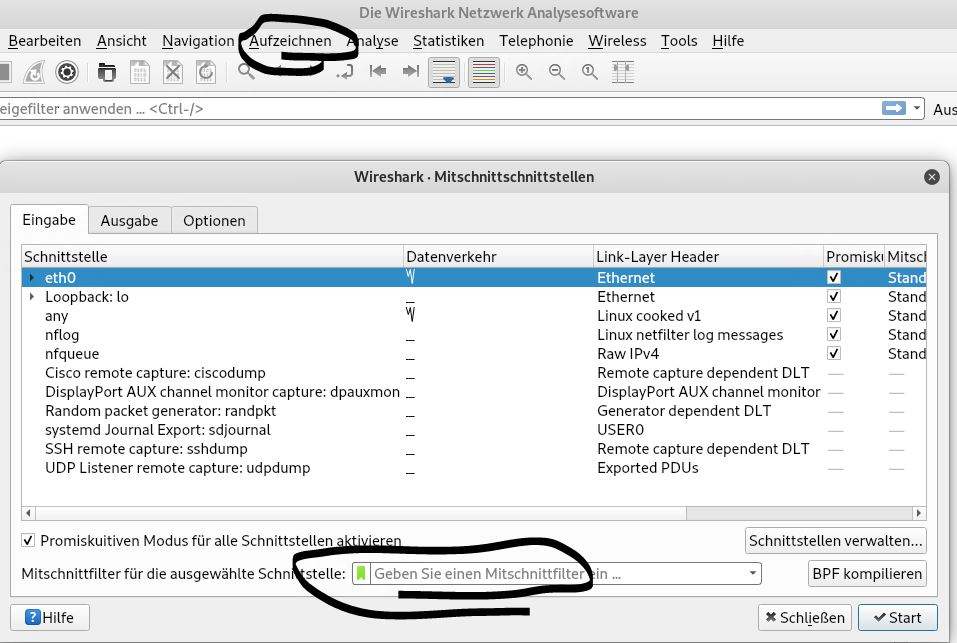
\includegraphics[width=0.7\textwidth]{./imgs/Picture1.jpg}
		\caption{Bild Filter-Aufzeichnung Wire-Shark}
		\label{fig:Bild1}
		
	\end{figure}
		
	% pfeile unter http://www.latex-pfeile.de/ || hierfür muss soweit ich es sehe kein Package eingebunden werden
	% einbindung Bild als Gleitbild: https://de.wikibooks.org/wiki/LaTeX-Kompendium:_Schnellkurs:_Grafiken
	\item Einfacher Mitschnittfilter auf host 8.8.8.8 mittels ping / ICMP\\
	{\sethlcolor{cyan}\hl{host 8.8.8.8}} \\
	{\sethlcolor{yellow}\hl{ping 8.8.8.8}} \\ 
	hier haben wir im Wire-Shark echo request und echo reply // geht hin und her zwischen srs \& destination. Somit wird nicht mehr der gesamte Traffic mitgeschnitten, sondern nur noch ein kleiner Teil, angepasst an unseren Filter.
	
	\item Erweiterter Mitschnittfilter auf host 8.8.8.8 mittels ping / ICMP nur auf den SRC(source) oder auf die DST(destination)  \\ 
	ist er zwar nicht fettaber der Umbruch funktioniert\\
	{\sethlcolor{cyan}\hl{dst host 8.8.8.8}} || {\sethlcolor{cyan}\hl{src host 8.8.8.8}} \\
	{\sethlcolor{yellow}\hl{ping 8.8.8.8}} \\ 
	hier werden nur die bestimmten Hosts analysiert, und nicht mehr die beiden Kommunikationsteilnehmer
\newpage	
	\item Filter auf DNS-Traffic via UDP   \\ 
	{\sethlcolor{cyan}\hl{port 53}} \\
	{\sethlcolor{yellow}\hl{dig @8.8.8.8 www.cbt-24.de A}} \\ 
	in der Konsole wir eine DNS anfrage erstellt mittels dig - dig ist sowas wie ein Frontend für den DNS-Service. im Wireshark sieht man die anfrage und die Response. DNS ist normalerweise immer über udp, da TCP erheblich aufwändiger ist. Das braucht ein einfache DNS Anfrage nicht. Dennoch zwinge ich im naechsten Beispiel das System einen TCP  handshake bei UDP zu machen\\
	
	\begin{figure}[htbp] 
		\centering
		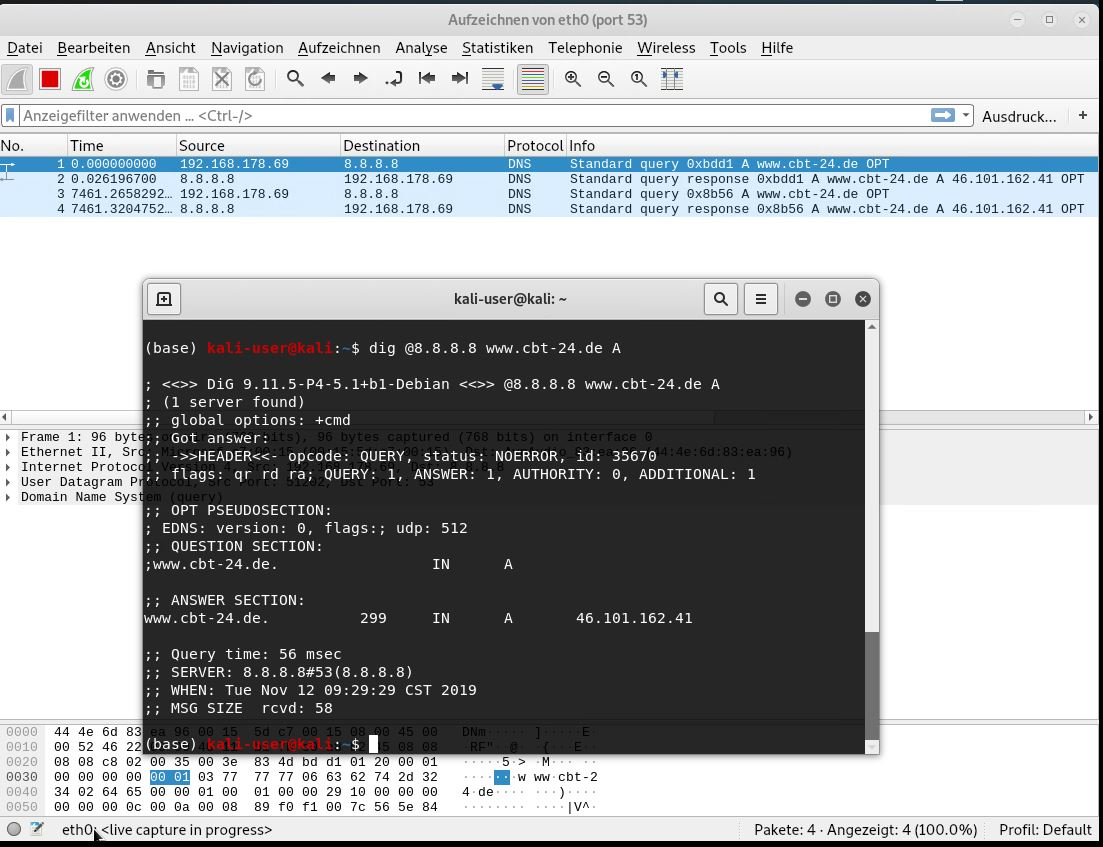
\includegraphics[width=0.7\textwidth]{./imgs/Picture3-Dig-DNS.JPG}
		\caption{DNS via UDP}
		\label{fig:Bild2}
		
	\end{figure}

	\item Filter auf DNS-Traffic via TCP   \\ 
{\sethlcolor{cyan}\hl{port 53}} \\
{\sethlcolor{yellow}\hl{dig @8.8.8.8 www.cbt-24.de A +tcp}} \\ 
Hier setzten wir eine DNS-Anfrage via UDP ab, hier sind erheblich mehr \\\
tcp Handshake \\
1) Client = Syn\\
2) Server = syn, ACK\\
3) Client = ACK\\
\begin{figure}[htbp] 
	\centering
	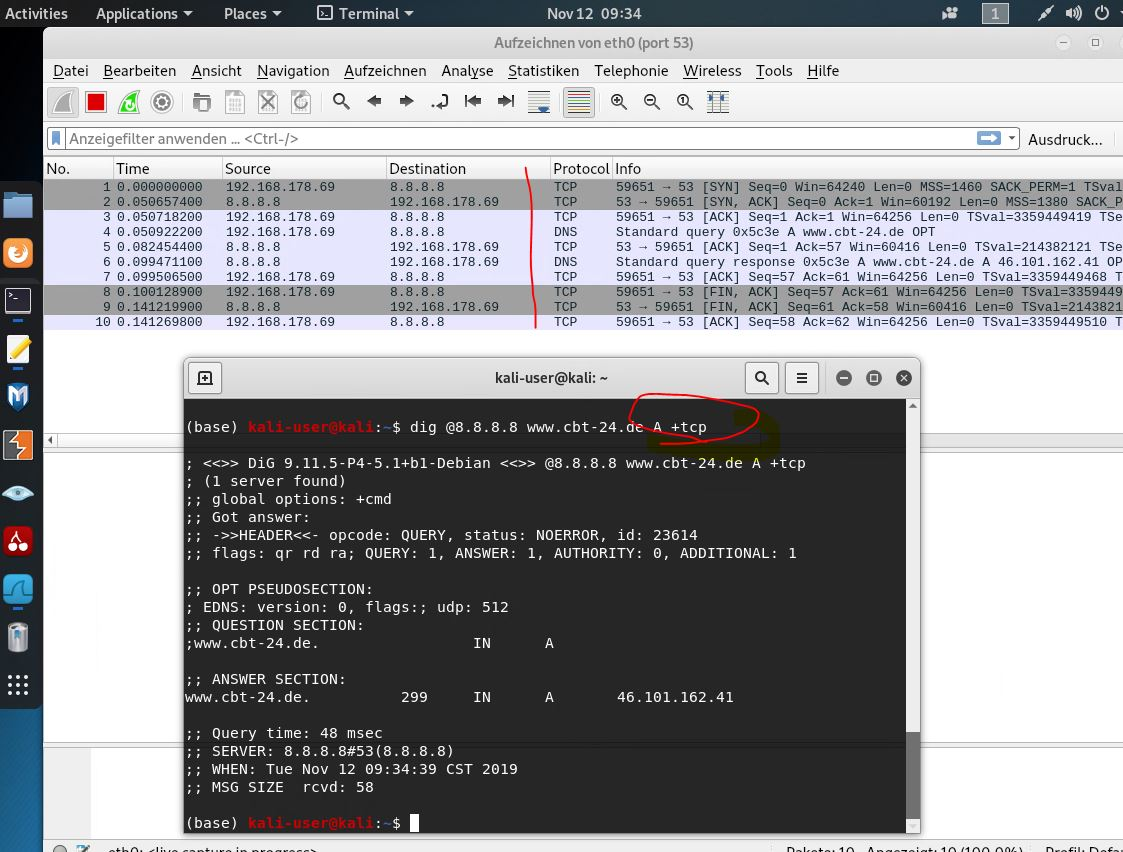
\includegraphics[width=0.7\textwidth]{./imgs/Picture3-Dig-DNS-tcp.JPG}
	\caption{DNS via TCP}
	\label{fig:Bild3}
	
\end{figure}
\\ wenn ich bei diesem Filte jetzt einen ICMP abfrage, schneidet es logischerweise nichts mit

	\item Filter auf DNS-Traffic auf einen bestimmten port  \\ 
	{\sethlcolor{cyan}\hl{port 53}} \\
	{\sethlcolor{yellow}\hl{dig @8.8.8.8 www.cbt-24.de A +tcp}} \\ 
	heir nur Traffic via Port 53
	
	\item Filter auf DNS-Traffic auf einen bestimmten port  \\ 
	{\sethlcolor{cyan}\hl{udp dst port 53}} \\
	{\sethlcolor{yellow}\hl{dig @8.8.8.8 www.cbt-24.de A +tcp}} \\ 
	hier nur den Traffic von udp \& dst 
	
	\item Filter auf DNS-Traffic auf einen bestimmten port mittels logischer Verknuepfungen  \\ 
	{\sethlcolor{cyan}\hl{udp dst port 53 and dst host 8.8.8.8}} \\
	{\sethlcolor{yellow}\hl{dig @8.8.8.8 www.cbt-24.de A +tcp}} \\ 
	hier die logischen Verknuepfungen, es werden nur Traffic zwischen google, via dns und udp, jetzt werden dns via udp anfragen die nicht auf 8.8.8.8 gehen nciht mitgeschnitten
	
	\item Filter auf DNS-Traffic auf einen bestimmten port mittels logischer Verknuepfungen  \\ 
	{\sethlcolor{cyan}\hl{udp dst port 53 and dst host 8.8.8.8 or dst host 192.168.178.1}} \\
	{\sethlcolor{yellow}\hl{dig @8.8.8.8 www.cbt-24.de A +tcp}} \\ 
	hier werden jetzt sowohl dns traffic zwichen google und lokalem Router mitgenschnitten, aber auch alle Packete von dst host 192.168.178.1 packages  $\Rightarrow$ or macht einen ganz neuen Filter auf
	
	\item Filter auf DNS-Traffic auf einen bestimmten port mittels logischer Verknuepfungen  \\ 
	{\sethlcolor{cyan}\hl{udp dst port 53 and (dst host 8.8.8.8 or dst host 192.168.178.1)}} \\
	{\sethlcolor{yellow}\hl{dig @8.8.8.8 www.cbt-24.de A +tcp}} \\ 
	jetzt entweder udp-Traffic von 8.8.8.8 oder on 192.168.178.1
	
	
	
	
\end{description}

\end{document}
